\newpage
\section{Implementation and Testing}\label{sec:testing}
Briefly alluded to in Section \ref{sec:system}, the simulation environment CyberSim is based on a SolidWorks modelling the rigid body dynamics of the Kobuki. The LabVIEW Robotics Environment Simulator solves ordinary differential equations (ODEs) for the dynamics of the system and renders the outcome into a display dialogue in 3D \cite{labguide}. Our envisioned state machine as mentioned in Section \ref{sec:FSM}, came to it's final states through multiple iterations. Regular testing of each design phase on the physical Kobuki brought our attention to issues that weren't obvious in theoretical planning or simulation.

\subsection{LabView vs. Microsoft Visual Studio (C/C++) and Eclipse}
\vspace{-0.2cm} LabView is the system engineering software produced by National Instruments to run the Kobuki obstacle course lab exercises. It provides a graphics user interface (GUI) approach to allow the user to drag and drop `blocks' into project surfaces and program visually. Microsoft Visual Studio (VS) is a standard integration development environment (IDE) that's used across the workplace for code development. The IDE comes with inbuilt compilers and debugger along with other software engineering basics such as automatic indentation and variable searching to ease coding. To run the code on the Kobuki, it would need to be transferred over into an Eclipse project file in order to connect to the Kobuki hardware. Both options allow simulation running CyberSim when the associated LabView software development kit (SDK) was downloaded and available.\\

To understand both implementation options better, the first MVP algorithm for obstacle avoidance was programmed using both LabView and VS/Eclipse. Figure \ref{fig:LabView} shows the CyberSim output indicating the state on a LabView state chart and Figure \ref{fig:VS} shows Visual Studio during a debugging session. To summarise this initial experiment, Table \ref{tab:labviewVSC} shows the key unique positives and negatives of both tools (comparison was made so that the negatives in one tool doesn't have a corresponding positive in the other tool). Clearly shown, VS and Eclipse offered more positives and less negatives than LabView. The unsolved reason to why the left bumper block wasn't usable in LabView was also a key reason why it was not chosen - without the left bumper sensor the Kobuki would fail to meet obstacle avoidance requirements when encountering any left obstacle. The main negative from Eclipse was the timeout, which was avoided by a ``TF" timeout override block in LabView. In week 10, the demonstrators shared the solution of writing \texttt{nohup} to override the TCP timeout before the binary execution on the Kobuki. In addition, instructions for wifi connection to the Kobuki was also given, which allowed faster testing and sharing of iterated code via local machine and GitHub repositories. Thence, the chosen implementation tool was Visual Studio and Eclipse.
\begin{figure}[H]
    \centering
    \begin{minipage}{0.45\textwidth}
    \centering
    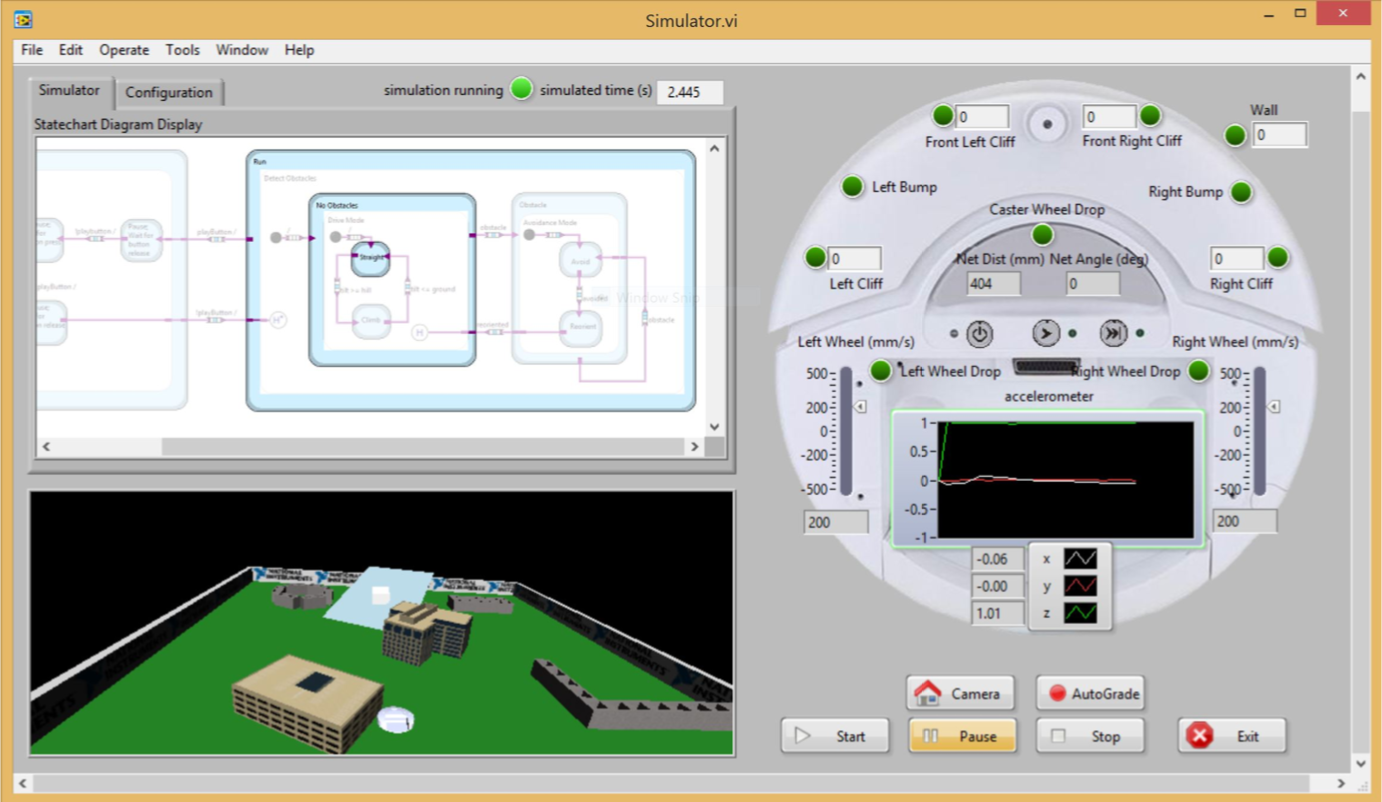
\includegraphics[width=8cm]{Images/LabViewStateChart.png}
    \caption{LabView statechart present in CyberSim for iRobot \cite[p.~32]{labguide}}
    \label{fig:LabView}
    \end{minipage} \hspace{0.5cm}% 
    \begin{minipage}{0.45\textwidth}
    \centering
    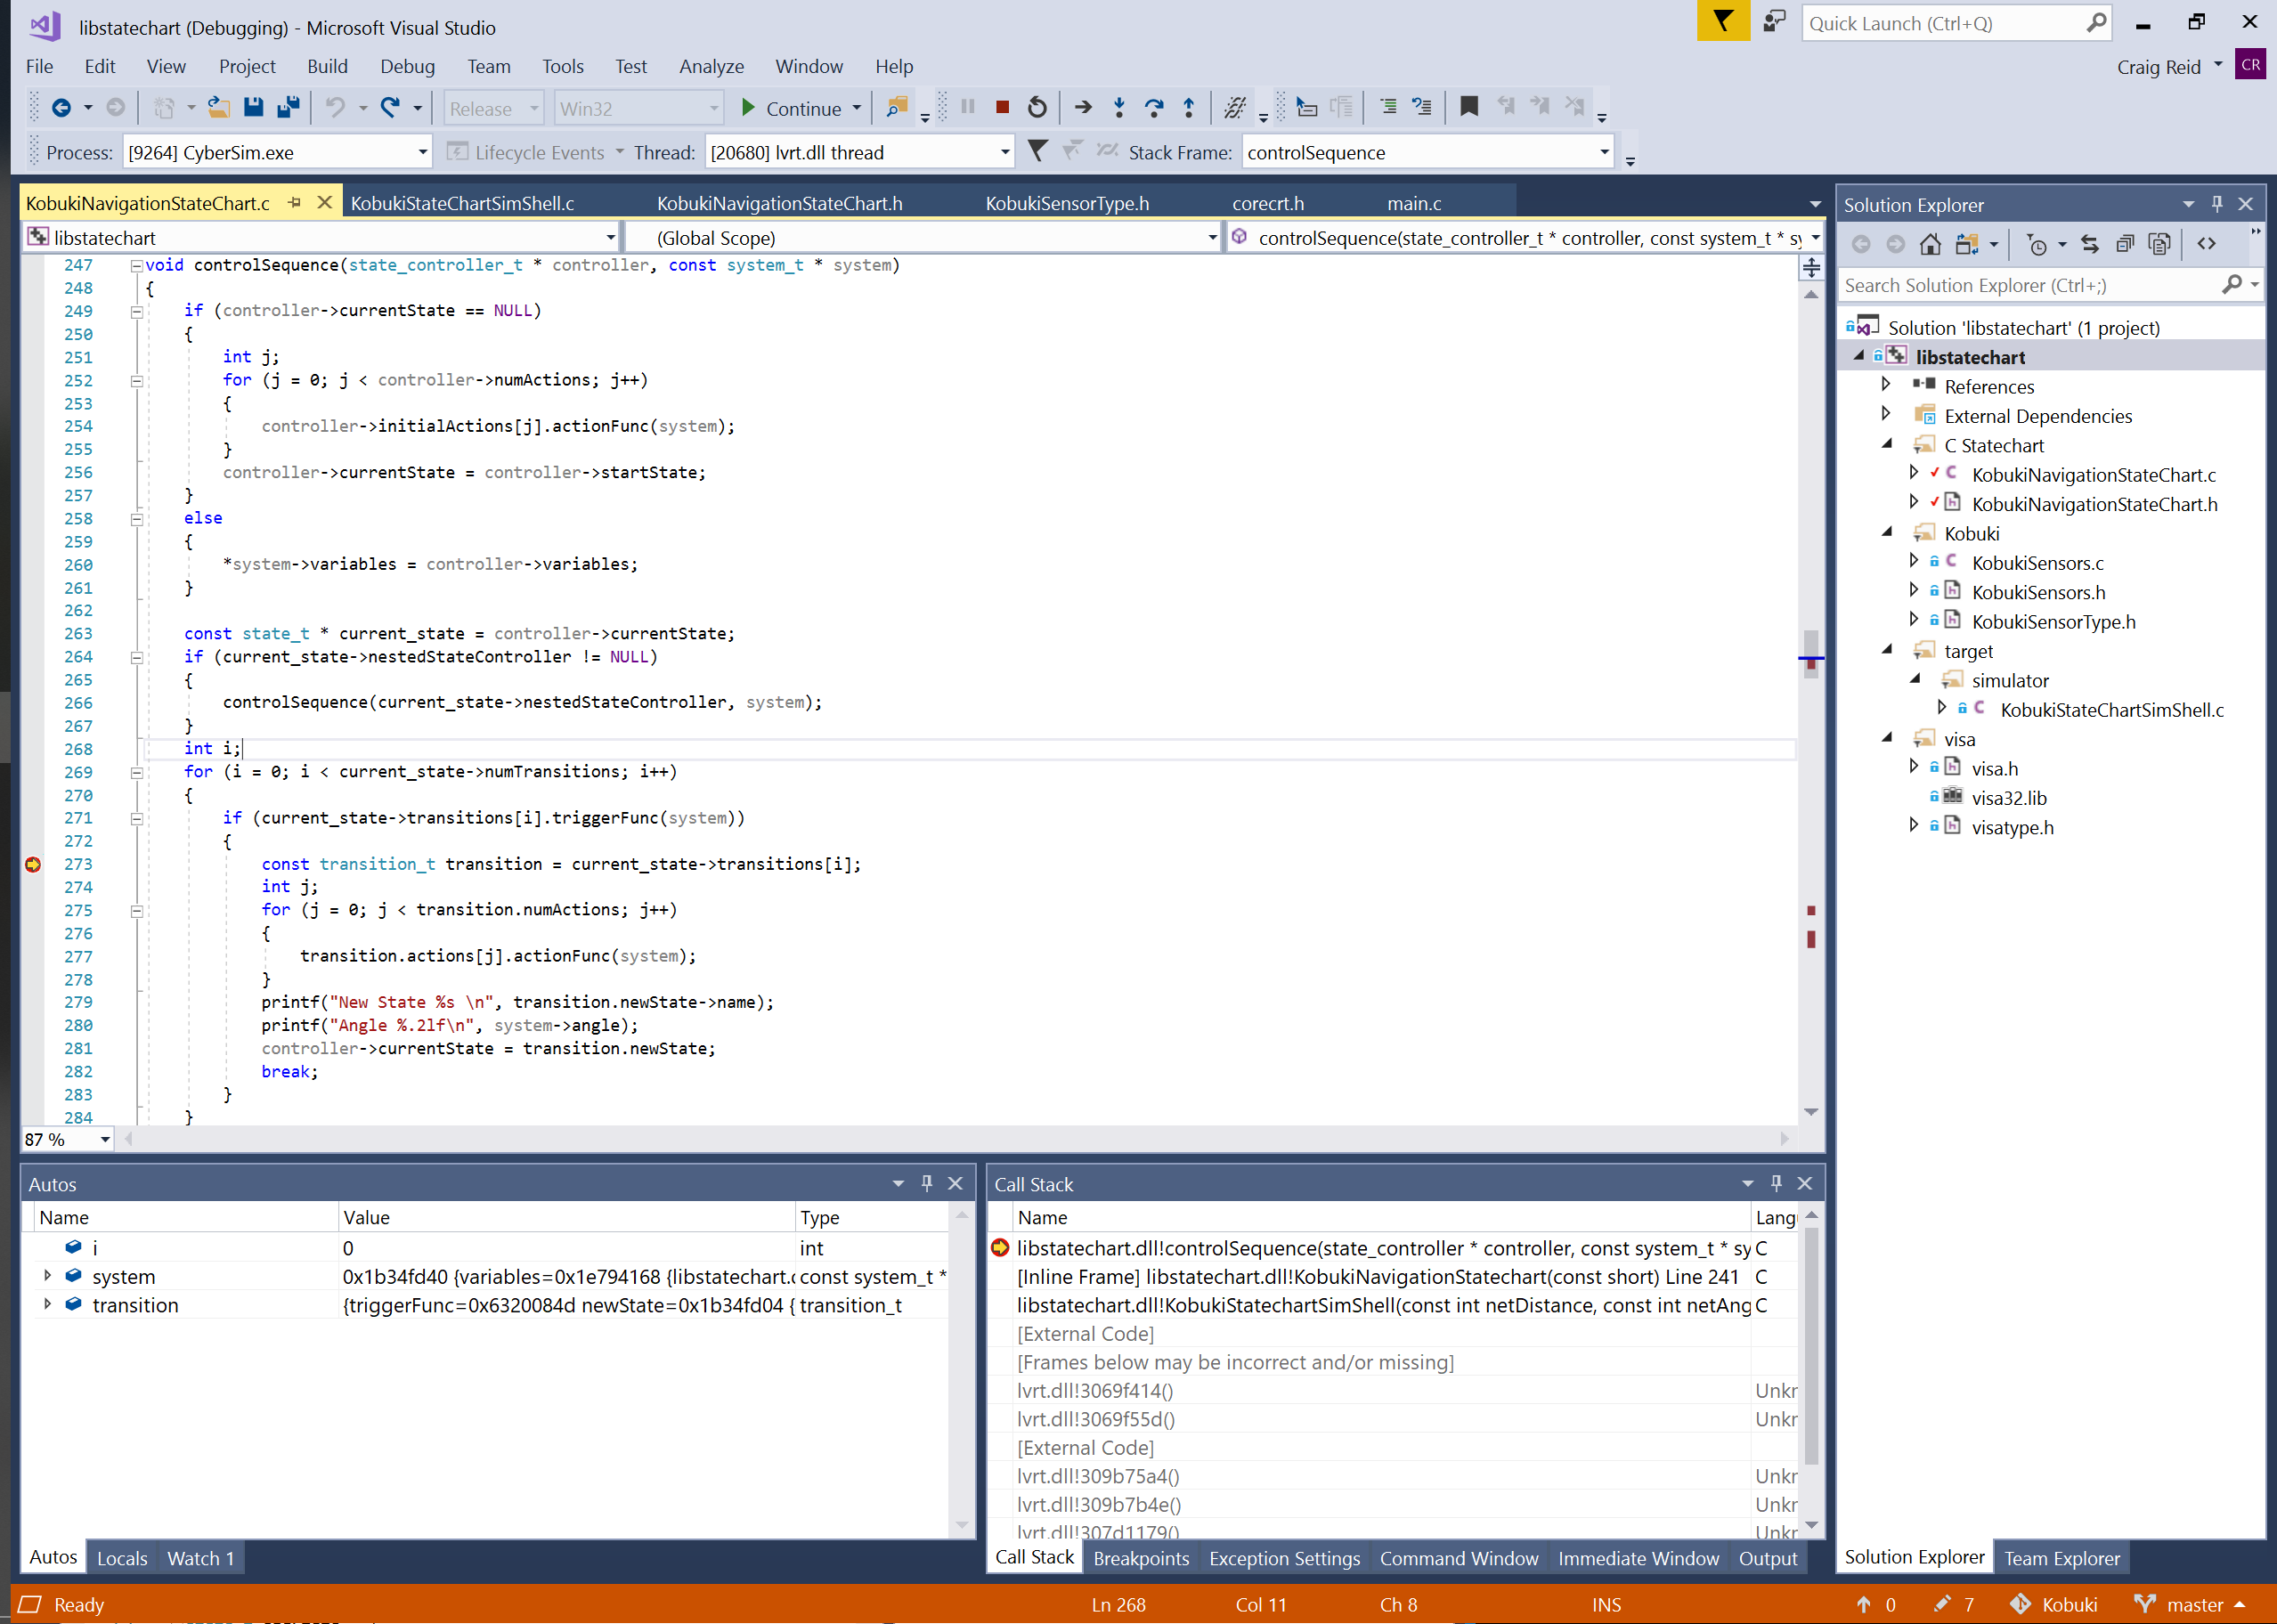
\includegraphics[width=8cm]{Images/VisualStudio.png}
    \caption{Visual Studio IDE connected to GitHub for source control for the project \texttt{libstatechart.sln}}
    \label{fig:VS}
    \end{minipage}
\end{figure}

\begin{table}[!ht]
    \centering
    \begin{tabularx}{\textwidth}{|X|X|}
        \hline
        \textbf{LabView} & \textbf{Visual Studio/Eclipse (C/C++)}\\
        \hline
        \begin{itemize}
            \item[+] Easy to visualise states and transitions
            \item[+] Code deployment onto Kobuki was very simple, it required only the single download button
            \item[+] CyberSim can show the states that the simulation traverses, thus allowing simple debugging
            \item[-] The LabView platform was often unstable and crashed three times unexpectedly without saving
            \item[-] Iteration of code was difficult to track all the different transition blocks that required to change
            \item[-] The GUI was not user friendly and was time consuming to individually select blocks and made sure lines fully connected
            \item[-] The use of variables wasn't very intuitive and required a lot of extra handling to initialise the variable abd add it individually to each transition
            \item[-] Repeated transitions or actions couldn't easily be reused and looks very convoluted
            \item[-] The Kobuki we used had a disabled left bumper which wasn't able to be controlled
            \item[-] Program was only accessible in the workshop sessions on the computers with LabView
        \end{itemize}
        &
        \begin{itemize}
            \item[+] Encouraged collaboration via GitHub to share the code and track changes or revert to previous versions when required
            \item[+] Debugging was very straightforward with standard error messages from the C compiler
            \item[+] Code written could include comments that described the process and provided more context behind the program
            \item[+] C offered execution efficiency with the variety of intuitive functions included in standard libraries and sped up the programming
            \item[+] All team members are experienced with coding in C and working on source code allowed contribution from both Windows and Mac users
            \item[-] Deployment on the Kobuki required a lot more steps to connect to a remote target, generate a binary and replace the original binary in the path and then execute via a terminal
            \item[-] Deployment on the Kobuki communicates using the TCP protocol and has a timeout
            \item[-] Configuration in Eclipse requires fiddly setup that may require starting from scratch if the machine is not already set up correctly
        \end{itemize}\\
        \hline
    \end{tabularx}
    \caption{Positives and negatives of LabView and Visual Studio/Eclipse}
    \label{tab:labviewVSC}
\end{table}

\subsection{Building a State Machine in C}
\vspace{-0.2cm} There are many ways to implement a state machine using C. There was a risk of having unmanageable and unreadable spaghetti code filled with conditional statements \cite{codingFSM}. The problem with using a conditional statement approach is the difficulty of seeing the difference between states, variables, triggers and actions as each state may require its independent variables to activate triggers and actions to capture dynamic history. A better approach defined states as structs and triggers/actions as function pointers \cite{structs_fnc_ptrs}. This means the main function only needs to look at the current state, check the triggers from the state and if any trigger returns true, perform the actions of that transition.\\

Once the core logic was implemented then adding states was as simple as creating a struct with function pointers to describe transitions. Functions that were commonly used such as calculating angles or checking for angle rotated were easily reused. Pointers offered a lot of flexibility in code development especially when iterating through new and uncertain approaches, such as how we were assessing the angles. An entire state only needed to change where the action pointed to if a new approach was tested in a new function without affecting other transitions. Furthermore, hierarchical state machines were easily implemented by allowing each state to contain another state. In practice, each refinement from the design (see Section \ref{sec:FSM}) was wrapped in a `controller' to handle the variables and behaviour (see Appendix \ref{app:code} to view source code).\\

Conditional statements were initially used for the MVP algorithm for obstacle avoidance, however, as complexity grew a new Git branch was created to use structs. Eventually the implementation proved so much easier and versatile that the structs branch was squash merged and replaced the original code. An example shown in Figures \ref{fig:DriveAvoidIfs}-\ref{fig:DriveAvoidStructs} compares the effort required between using switch case/conditional statements and structs/function pointers for implementing the extra \textit{ReverseCorner} state from the \textit{DriveAvoid} state. This was our third iteration for developing the obstacle avoidance algorithm in Section \ref{sec:obstacle_alg}. Blue indicates what's already present in the obstacle avoidance, yellow shows reused functions, three Figure \ref{fig:DriveAvoidStructs} there are only a total of three states at the end of the implementation and reusing existing functions was easy by swapping the left and right functions being pointed to. The end of the if statement changes in Figure \ref{fig:DriveAvoidIfs} shows little connection to what was used already and shows a total of five states with overlapping behaviours to the original code for \texttt{DriveAvoid}. What continues after the two new \textit{CornerTurn} states are also be even more nested in if statements.\\
\begin{figure}[H]
    \centering
    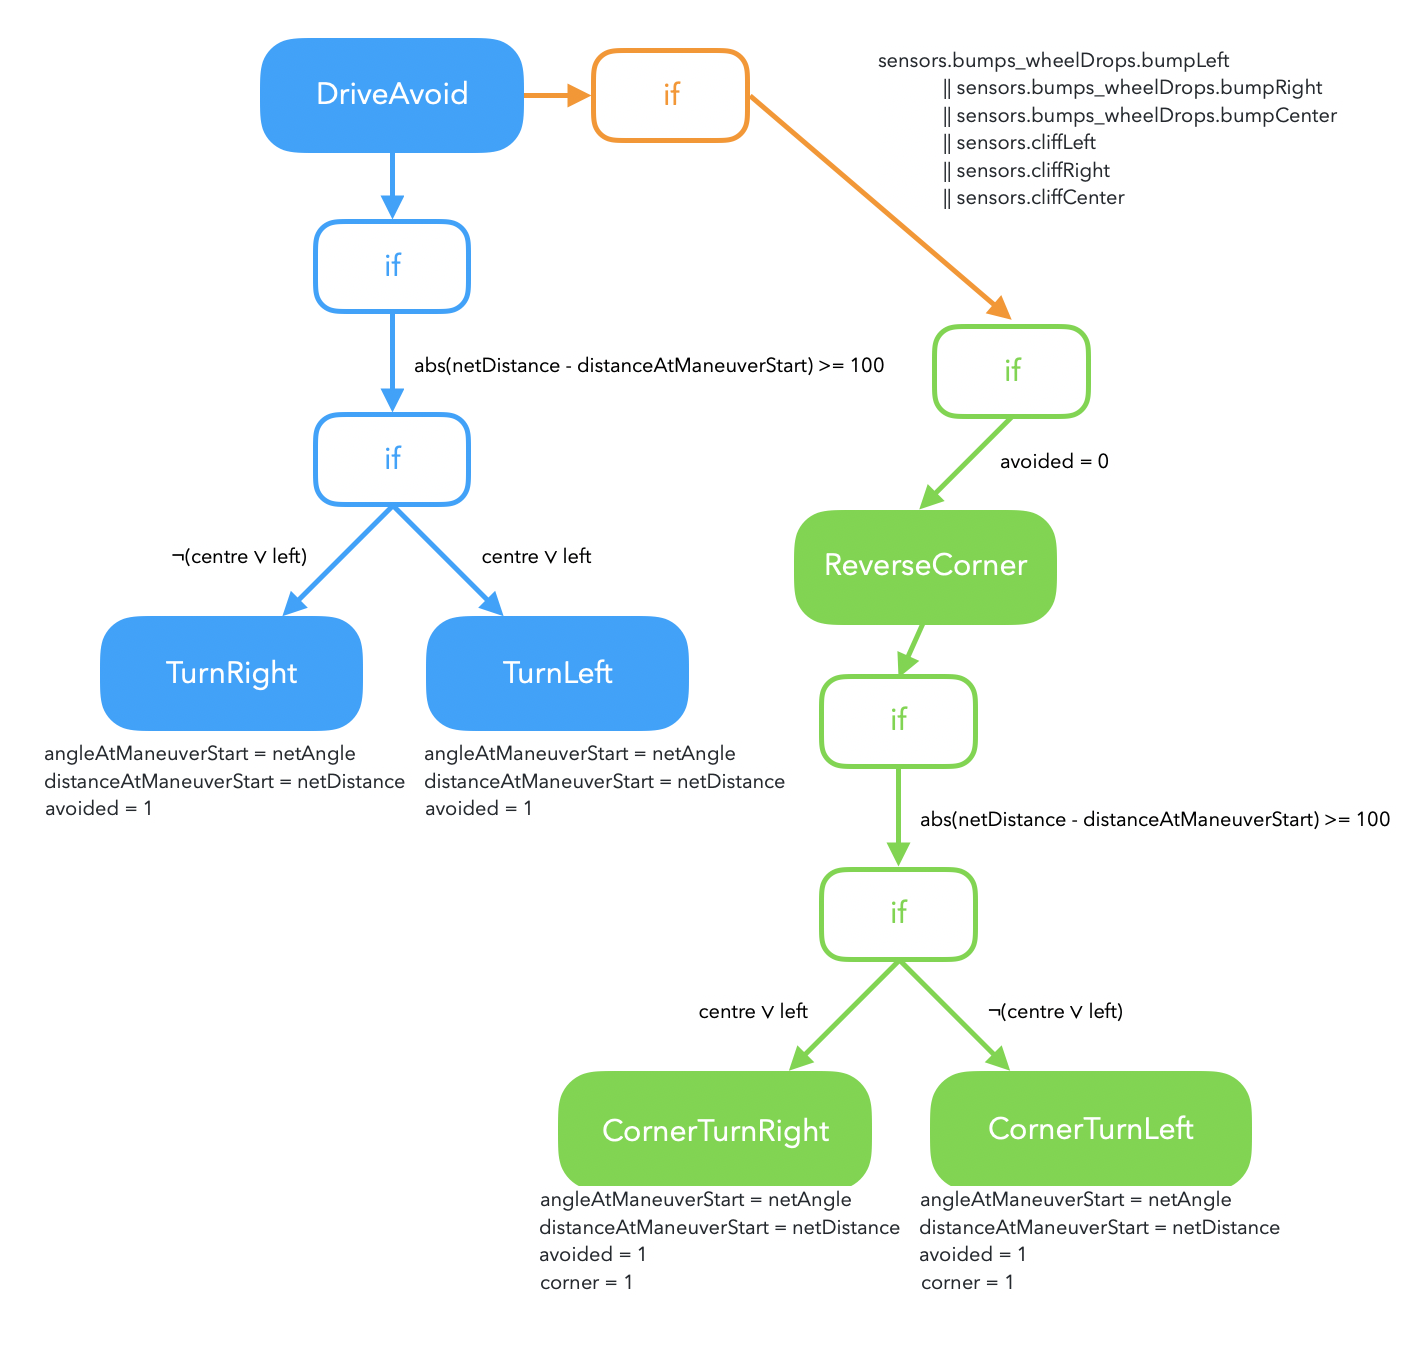
\includegraphics[width=12cm]{Images/DriveAvoidIfs.png}
    \caption{Flowchart describing three new if conditions and two new states added to existing conditional statements}
    \label{fig:DriveAvoidIfs}
\end{figure}
\begin{figure}[H]
    \centering
    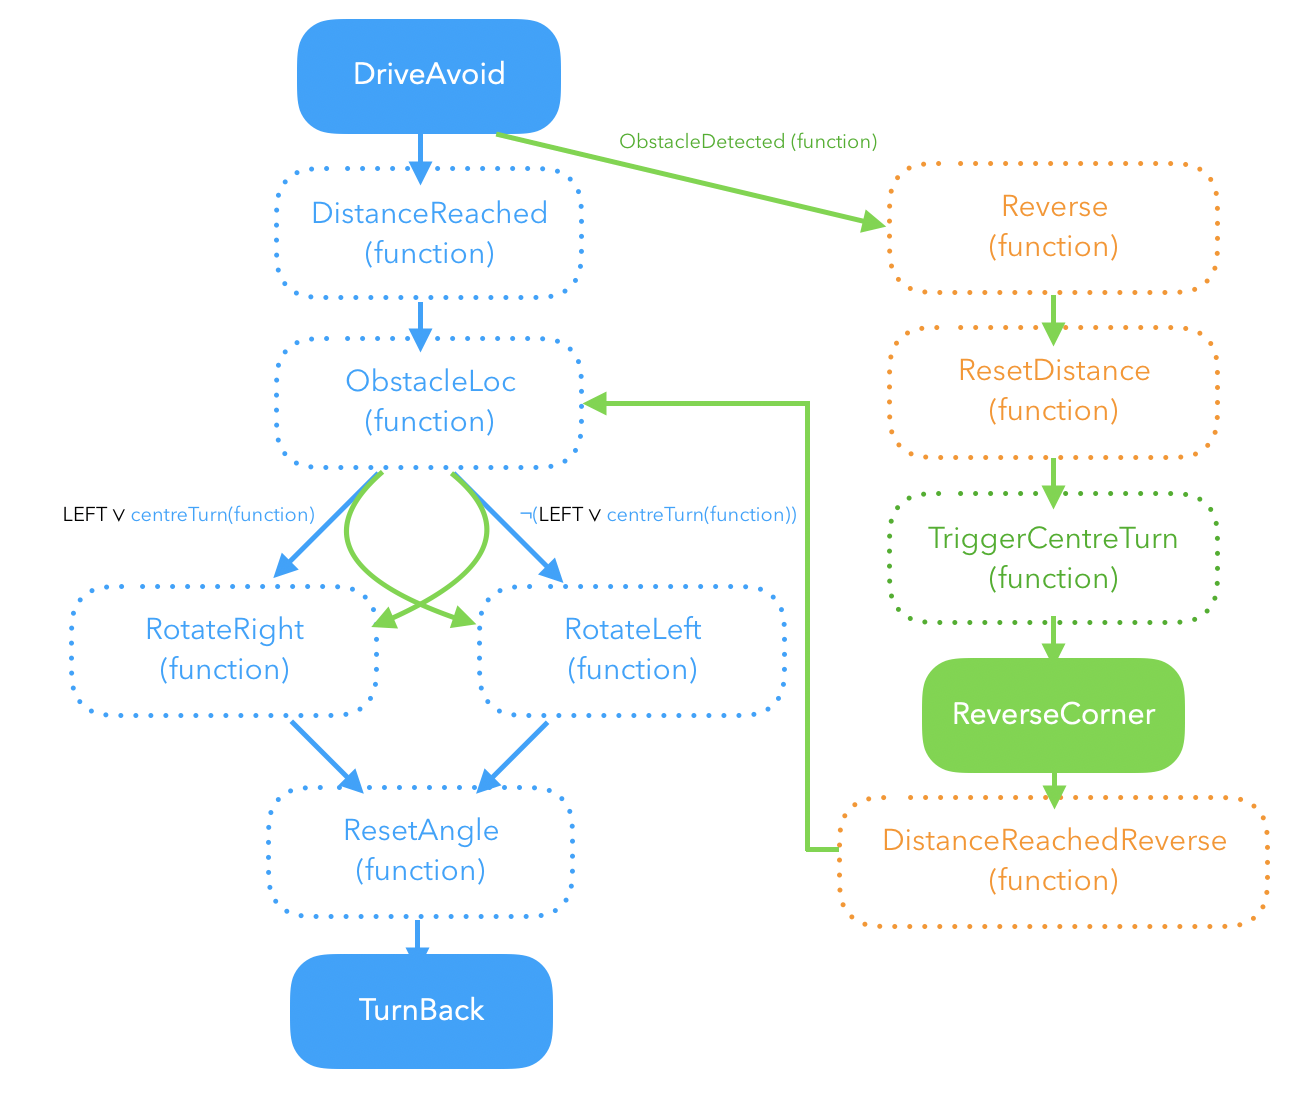
\includegraphics[width=11cm]{Images/DriveAvoidStruct.png}
    \caption{Flowchart describing one new function and one new state added to existing transitions}
    \label{fig:DriveAvoidStructs}
\end{figure}

% Simulation results, and how the simulation was shit.
\subsection{Simulation using CyberSim}\label{sec:cybersim}
\vspace{-0.2cm} The simulation environment determines noise behaviours through random numbers, which means that each Kobuki test trace will never be exactly the same. Being non deterministic is beneficial when testing as it better emulates a real world situation as environmental factors that influence outcomes will always change \cite{labguide}.\\

CyberSim was helpful in testing obstacle avoidance and the development iterations concluded with satisfactory results. The ability to increase speeds to simulate the robot faster was useful sometimes e.g. when quickly testing the change for different bumpers leading to different turn directions. The \texttt{Navigation Maze} environments were very effective in testing the \textit{ReverseCorner} state in the last development iteration. The first try successfully demonstrated the robot turning around the opposite way from the second obstacle but when hitting the centre bumper again the turning direction (initially \texttt{centreTurn = false} and will turn left) did not change although the function \texttt{ToggleCentreTurn()} had reset the variable (when encountering an obstacle during \textit{DriveAvoid}, \texttt{centreTurn = true} and will turn right). Troubleshooting this concluded that system variables were always reset to the initial default upon state change despite the function being executed. This was a flaw in the implementation of the core hierarchical extended state machine system. The solution was to make the \texttt{centreTurn} variable a global variable to override the reset and this worked in simulation.\\ 

Despite successes in obstacle avoidance, CyberSim was not the best simulation environment for hill climb. Some key issues with the solutions or alternative tests are expressed in Table \ref{tab:cybersim_hillclimb} and Figure \ref{fig:cybersim_hillclimb} shows the Kobuki in CyberSim whilst on an incline in \texttt{Environment - south ramp left}. Through what was successfully simulated in CyberSim, a key conclusion was that the hill climb MVP algorithm, which used raw accelerometer angles to detect incline and reorient directly towards uphill and downhill, did not produce reliable behaviours. This therefore led to the second iteration, which used angle calculation from the accelerometer readings (see Section \ref{sec:hill_alg}). Testing this in CyberSim saw the robot detecting and reorienting being less affected by accelerometer reading fluctuations.
\begin{table}[H]
\centering
\begin{tabularx}{\textwidth}{|X|X|}
    \hline
    \textbf{Key Issue in CyberSim Hill Climb} & \textbf{Solution or Alternative Tests}\\
    \hline
    The slope on simulation environments e.g. \texttt{Environment - south ramp left}, is not tilted via a single axis and there wasn't a clear way to visually confirm whether the robot was driving directly uphill or downhill. 
    & 
    Meticulous observation of the thresholds and angles with used to calibrate the testing. Implementation on the physical Kobuki was always used to confirm behaviours.\\
    \hline
    Incline thresholds were different to test ramp used for testing in the workshops. Simulation thresholds were very small and visually there wasn't a good way to tell if the hill climb states were active. The accelerometer readings also suffered a lot from fluctuations, where randomised noise produced non-deterministic confusing outcomes.
    &
    The code included an \texttt{isSimulator} variable to toggle between the real and simulator thresholds. Again, implementation on the physical Kobuki was necessary to confirm incline detection.\\
    \hline
    The Kobuki in simulation had the accelerometer directions swapped for the $\pm y$ and $\pm x$ axis.
    &
    \texttt{isSimulator} also triggered a different yaw angle $\psi$ calculating formula (see Section \ref{sec:acc}).\\
    \hline
    The environment did not offer a plateau to test middle flat state during hill climb.
    & 
    Testing on a plateau in real life was used to confirm Kobuki behaviours.\\
    \hline
    CyberSim does not have the same 'pause' function as the B0 button. Even though the button can be pressed on the GUI, what is outputted is only a simulation pause and overrides any state changes \cite[p.~33]{labguide}.
    &
    The play/pause states were tested on the physical Kobuki whilst testing hill climb. B0 button was pressed to start the Kobuki, pause and unpause it.\\
    \hline
\end{tabularx}
\caption{Issues and Solutions or Alternatives whilst using CyberSim for testing Hill Climb algorithms}
\label{tab:cybersim_hillclimb}
\end{table}
\begin{figure}[H]
    \centering
    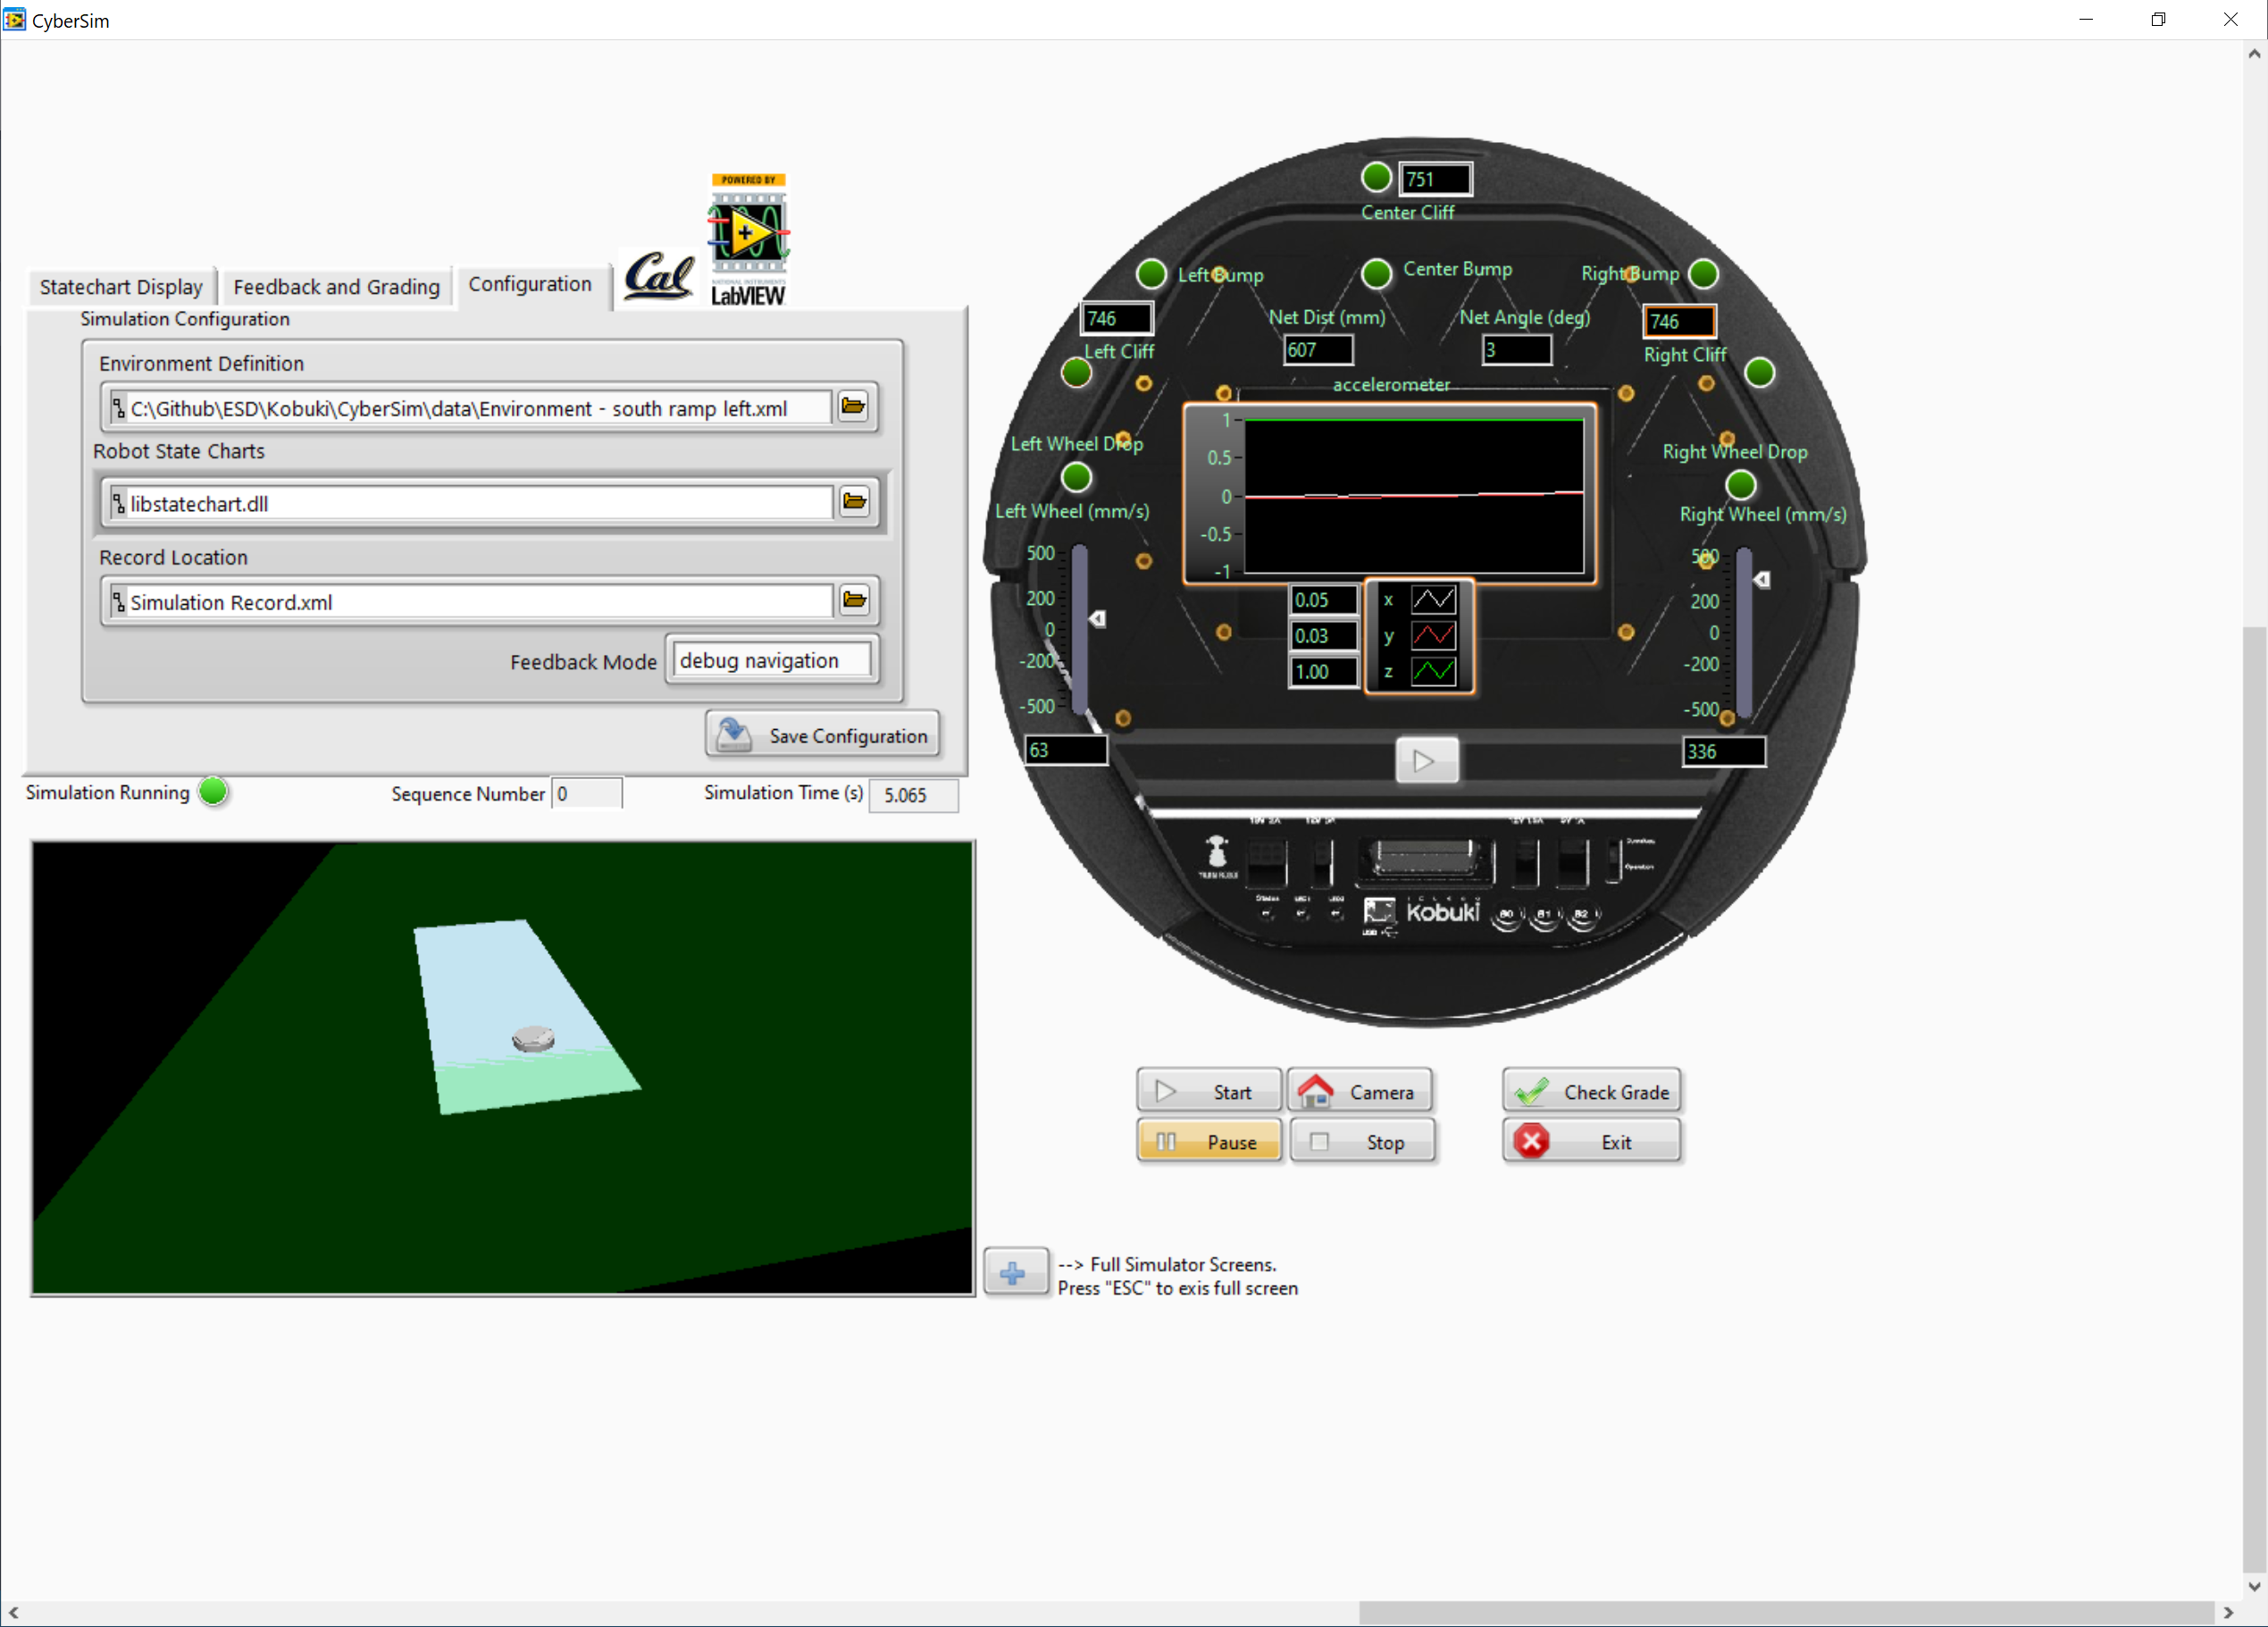
\includegraphics[width=14cm]{Images/CyberSimSlope.png}
    \caption{Showing the Kobuki in CyberSim on an incline and the small $x$ and $y$ values}
    \label{fig:cybersim_hillclimb}
\end{figure}

\subsection{Kobuki Testing}\label{sec:hill_test}
\vspace{-0.2cm} When testing the obstacle avoidance algorithms on the Kobuki the realisation was that speed was a factor in the accuracy of turning. The final speed was set to \texttt{200} (mm/s) with the intention to make the Kobuki respond relatively fast to complete the obstacle course on time and remain within an accurate range. The wheeldrop sensors were also debated whether to leave in the algorithm as it seemed to pick up minor lifts and trigger obstacle avoidance states. At the end it was decided that the wheeldrop sensors were to remain in obstacle detection as it was a project requirement that the Kobuki remained touching the ground.\\

Hill climb saw the benefits of slower speed on the ramp as well as higher speeds seemed to drive the wheels a lot more and cause the wheels to lift thereby activating the wheeldrop sensors. Using a separate set of thresholds, the incline detection was tuned to be above 0.2 radians ($11.5^\circ$) to allow significant room for fluctuations. Descending angles were also treated for wrapping the calculated results bewteen $\pm 180^\circ$ as the initial trials showed the Kobuki turning back up when the values remained positive on descent. In the \textit{Descending} state, if the calculated \texttt{angle} was greater than 0, $\pi$ was subtracted, otherwise $\pi$ was added. Testing this in week 10 after wifi connection was enabled allowed the angle values and states to be printed in the Eclipse terminal, which meant spotting the error and seeing the correction was very quick. The Eclipse printed outputs can be seen in Figure \ref{fig:eclipse_output}.\\

A final development was fine tuning the chattering during orientation. Implementing a feedback loop to turn a percentage of the measured offset angle saw the Kobuki glide through the tested inclines smooth without stutter. A full test sequence of state outputs from terminal can be seen in Appendix \ref{app:hill_states}. The terminal outputs indicate the implemented hill climb algorithm being able to achieve incline detection moving from \textit{Drive} to \textit{Ascending} and also detecting cliffs and triggering obstacle avoidance states as well as \textit{Descending} and finishing on flat ground on \textit{End}. Whilst testing hill climb, the state outputs from pausing and unpausing were also successful and are captured in Appendix \ref{app:play_pause_states}.
\begin{figure}[H]
    \centering
    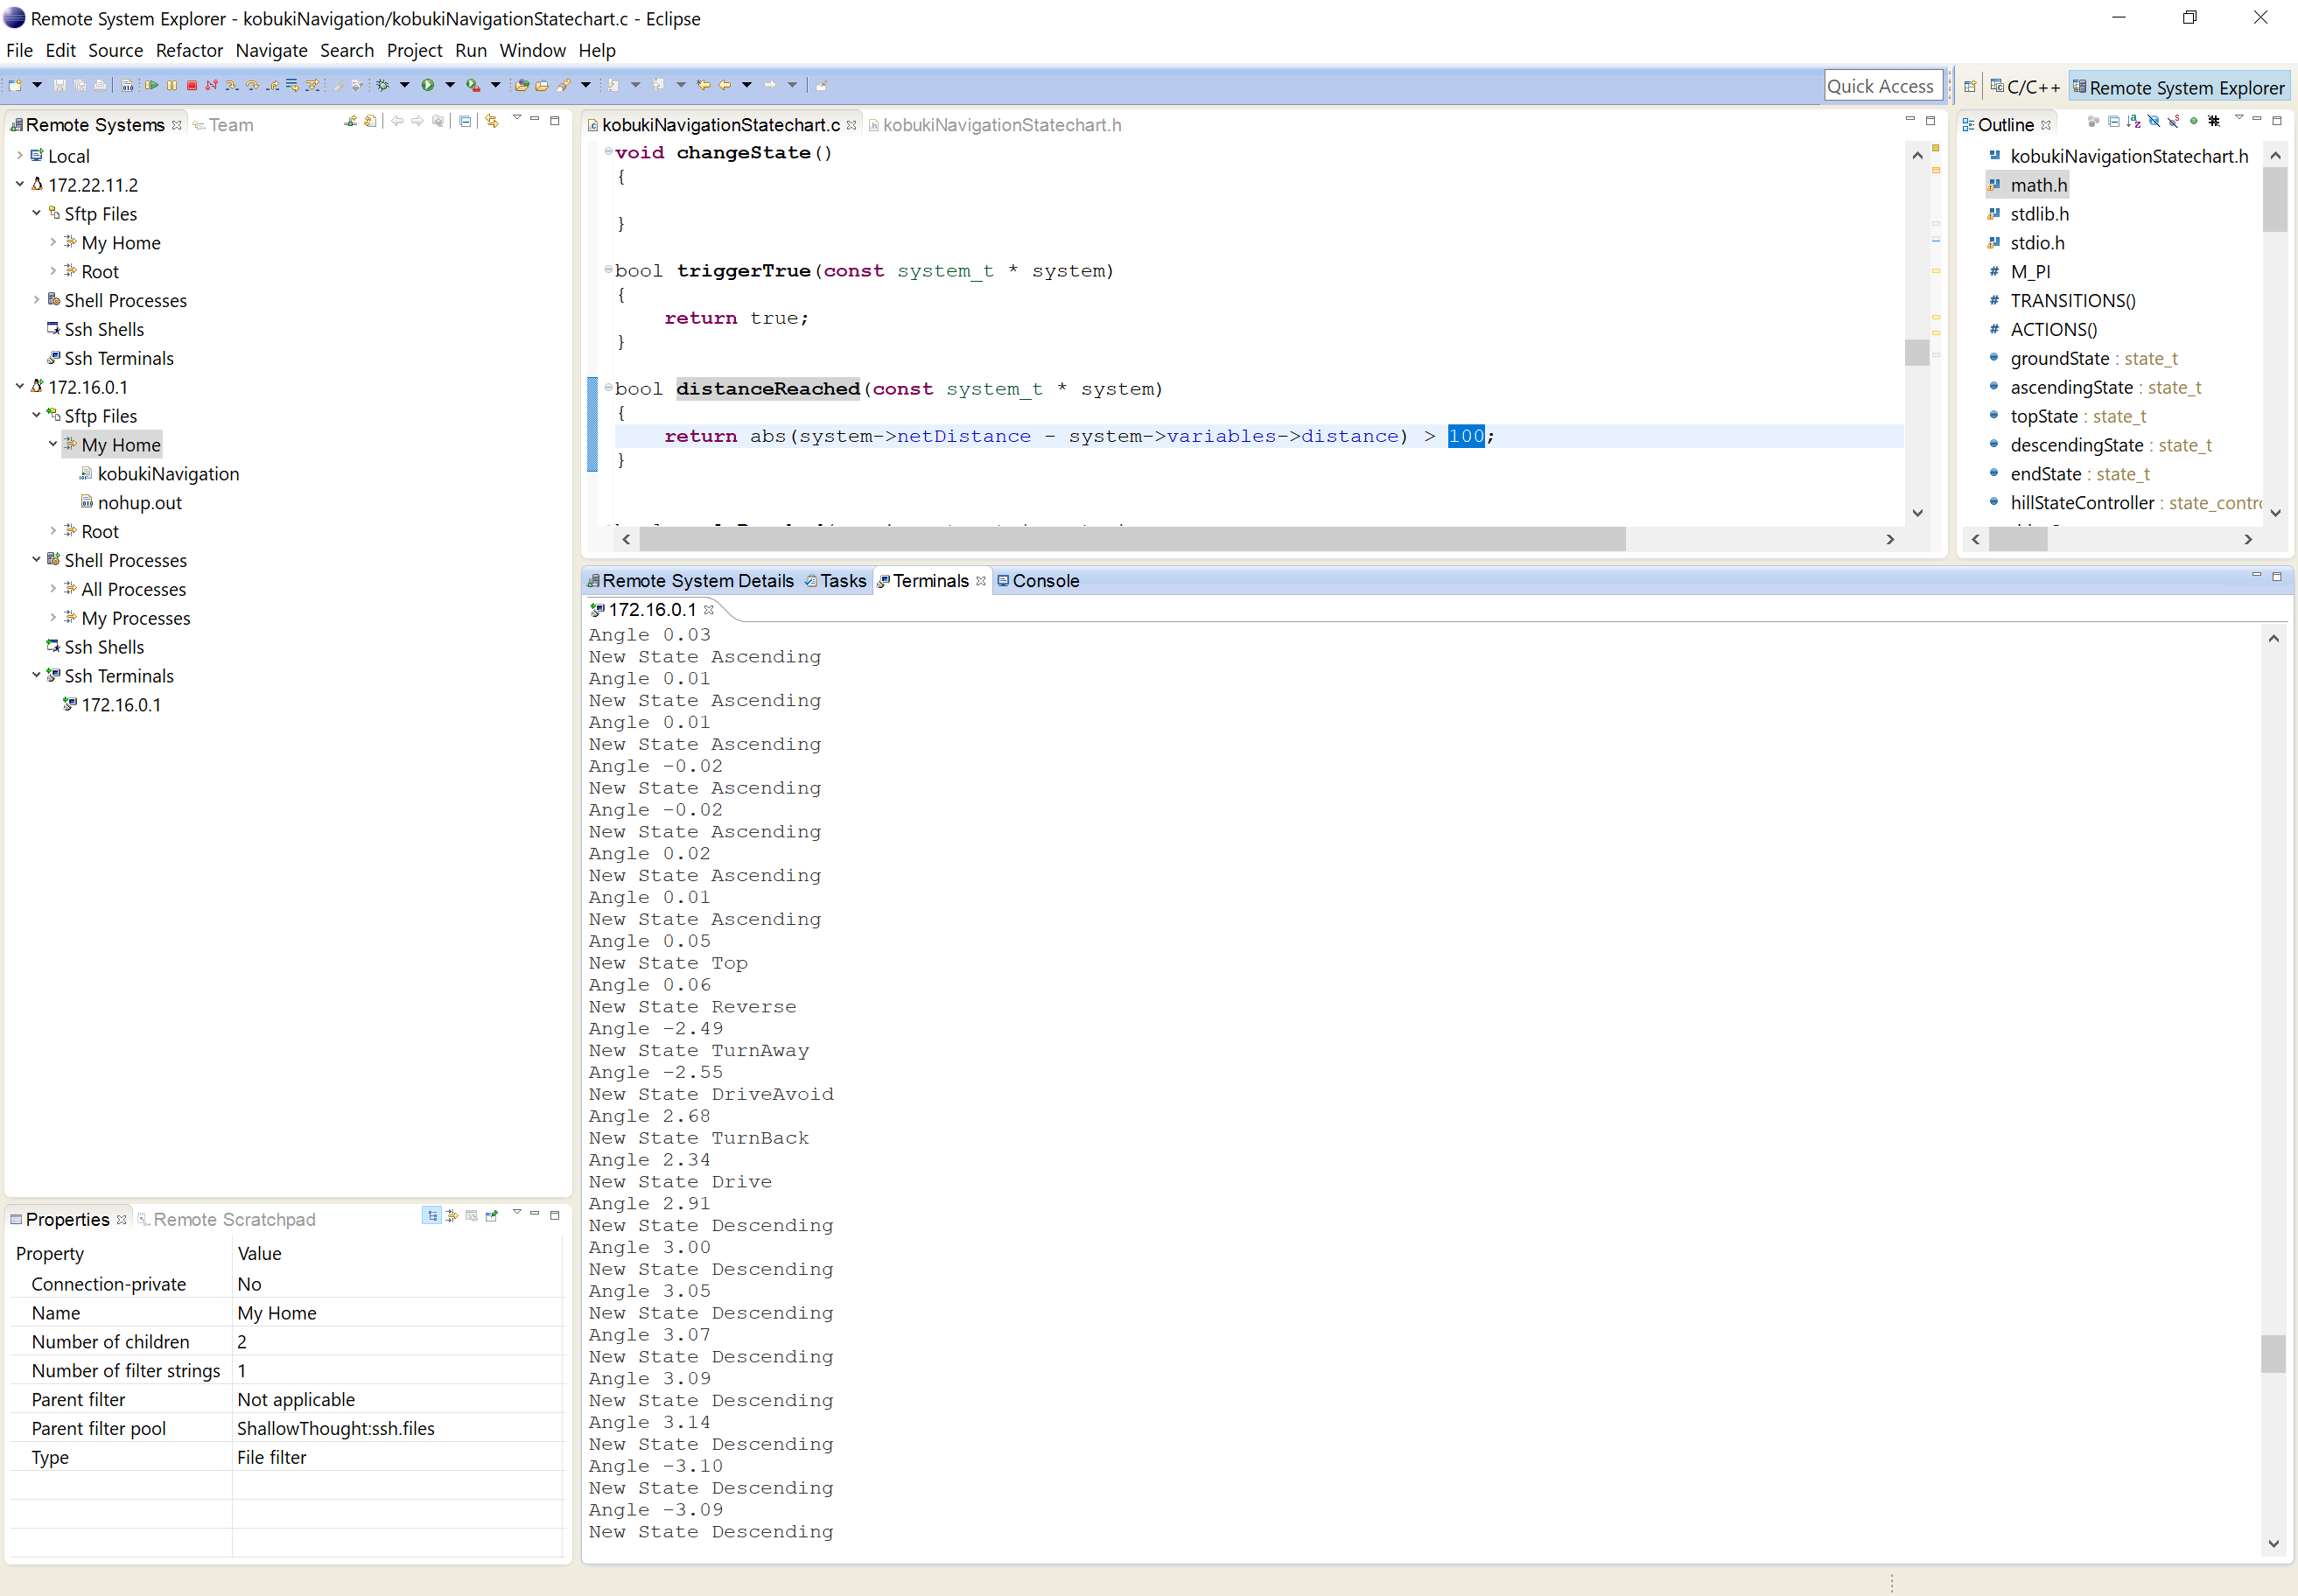
\includegraphics[width=15cm]{Images/eclipse_screenshot.PNG}
    \caption{The real time output showing calculated descent angles (rad) and states in the Eclipse terminal}
    \label{fig:eclipse_output}
\end{figure}